\chapter{Caso de estudio}
\label{cap:caso_de_estudio}
En el presente capítulo se analizará el caso de estudio para el cual se aplicará el Sistema Jigsaw Coding. En primer lugar se describirán los temas sobre los que estará basado la sesión jigsaw que será desarrollada usando el sistema web desarrollado. Posteriormente se describirá cómo están formados los grupos expertos y grupos jigsaw y finalmente se explicará brevemente la fase de evaluación para la sesión jigsaw.

\section{Definición del caso de estudio}
El caso de estudio para la aplicación del Sistema Jigsaw Coding consta principalmente de estudiantes de las escuelas profesionales de Sistemas y Software de la Universidad Nacional Mayor de San Marcos en cuyas carreras llevan o han llevado cursos relacionados a Programación y Algoritmos. \\

La muestra consta de 41 alumnos divididos en dos grupos: Grupo Sistemas(26 alumnos) y Grupo Software(15 alumnos). En el Grupo Sistemas se realizó un sorteo para determinar a los alumnos que formarían parte del grupo de control al cual solamente se le aplicaría la evaluación y no pasaría por la fase expertos y la fase jigsaw. El objetivo de formar un grupo control es básicamente para poder evaluar los beneficios que la técnica colaborativa jigsaw brinda en el aprendizaje, y en este caso, en la resolución de problemas de programación.\\

De esta forma, el Grupo Sistemas Principal estuvo formado por 16 alumnos y el Grupo Sistemas Control se formó con 10 alumnos. Este mismo proceso se realizó para el Grupo Software obteniendo asi un Grupo Software Principal con 9 alumnos y un Grupo Software Control de 6 integrantes. Ver figura \autoref{fig:c5_poblacion}\\

\begin{figure}
	\centering
	\caption{Población del caso de estudio.}
	\label{fig:c5_poblacion}
	\fbox{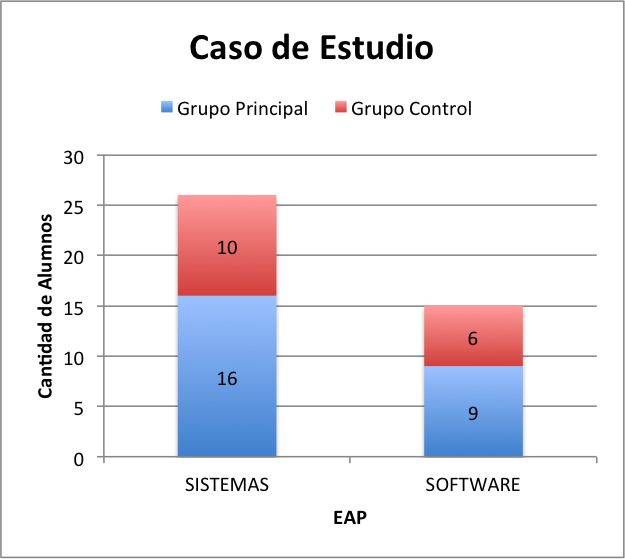
\includegraphics[scale=0.4]{figuras/chapter05/poblacion}}
\end{figure}
\newpage
\section{Definición de temas para el caso de estudio}
\label{sec:problemas}
Para este caso de estudio, se prepararon problemas para evaluar a los alumnos en cuanto a su conocimiento sobre operadores($+,-,x,/, mod$), estructuras condicionales, recursividad y ordenamiento.

\subsection{Problemas}

%%es triaungulo, fibonacci, segundos, burbuja ascendente.
%%ordernar abc, factorial, burbuja descendente
Durante la fase de expertos y fase jigsaw se usaron los siguientes problemas:

\begin{enumerate}
	\item \textbf{Segundos}. Elabore un programa que convierta un número de n segundos en horas minutos y segundos. Ejemplo: 100 segundos es 0 h 1 min 40 seg.
	\item \textbf{Es triángulo}. Determinar si un triángulo es: equilátero, isósceles o escaleno, conociendo sus tres lados (a,b,c).
	\item \textbf{Fibonacci}. La serie de Fibonacci comienza con un 0, luego un 1 y a partir de ahí cada número es la suma de los dos anteriores. Elabore un programa recursivo para mostrar los 10 primeros números de la serie de Fibonacci.
	\item \textbf{Burbuja ascendente}. Usando el algoritmo Bubble Sort ordenar en forma ascendente el siguiente array de enteros: 50,26,7,9,15,27.
	
\end{enumerate}

Para la fase de evaluación se elaboró un examen con los siguientes problemas, que dicho sea de paso, son bastante parecidos a los ya mostrados en las fases de expertos y jigsaw.

\begin{enumerate}
	\item \textbf{Ordenar a,b,c}. Implementar una programa que dados tres números a, b y c, los devuelva ordenados de menor a mayor.
	\item \textbf{Factorial}. Elaborar un programa que calcule el factorial de un número n usando recursividad. ($n <= 5$ ).
	\item \textbf{Burbuja descendente}. Usando el algoritmo Bubble Sort ordenar en forma descendente el siguiente array de enteros: 50,26,7,9,15,27.
\end{enumerate}

\section{Aplicación del Sistema Jigsaw Coding al caso de estudio}

En la figura \ref{fig:c5_poblacion} se puede ver la cantidad de alumnos para cada grupo definido. Naturalmente, se crearon 4 sesiones jigsaw en el sistema JigsawCoding a las cuales se asignaron los respectivos alumnos de Sistemas y Software, tanto para los grupos principales como para los grupos control. Estos últimos, solo fueron asignados para que realicen el examen de la fase evaluación, el cual fue igual para todos los 41 alumnos del caso de estudio.

Para el Grupo Sistemas Principal el sistema JigsawCoding formó de manera aleatoria los 4 grupos expertos y 4 grupos jigsaw a los cuales posteriormente se les asignó los problemas: Segundos, Es triángulo, Fibonacci y Burbuja ascendente. La composición de cada grupo puede verse en la figura \ref{fig:c5_sistemas_grupos}.

\begin{figure}[!h]
	\centering
	\caption{Grupos Expertos y Grupos Jigsaw - EAP Sistemas}
	\label{fig:c5_sistemas_grupos}
	\fbox{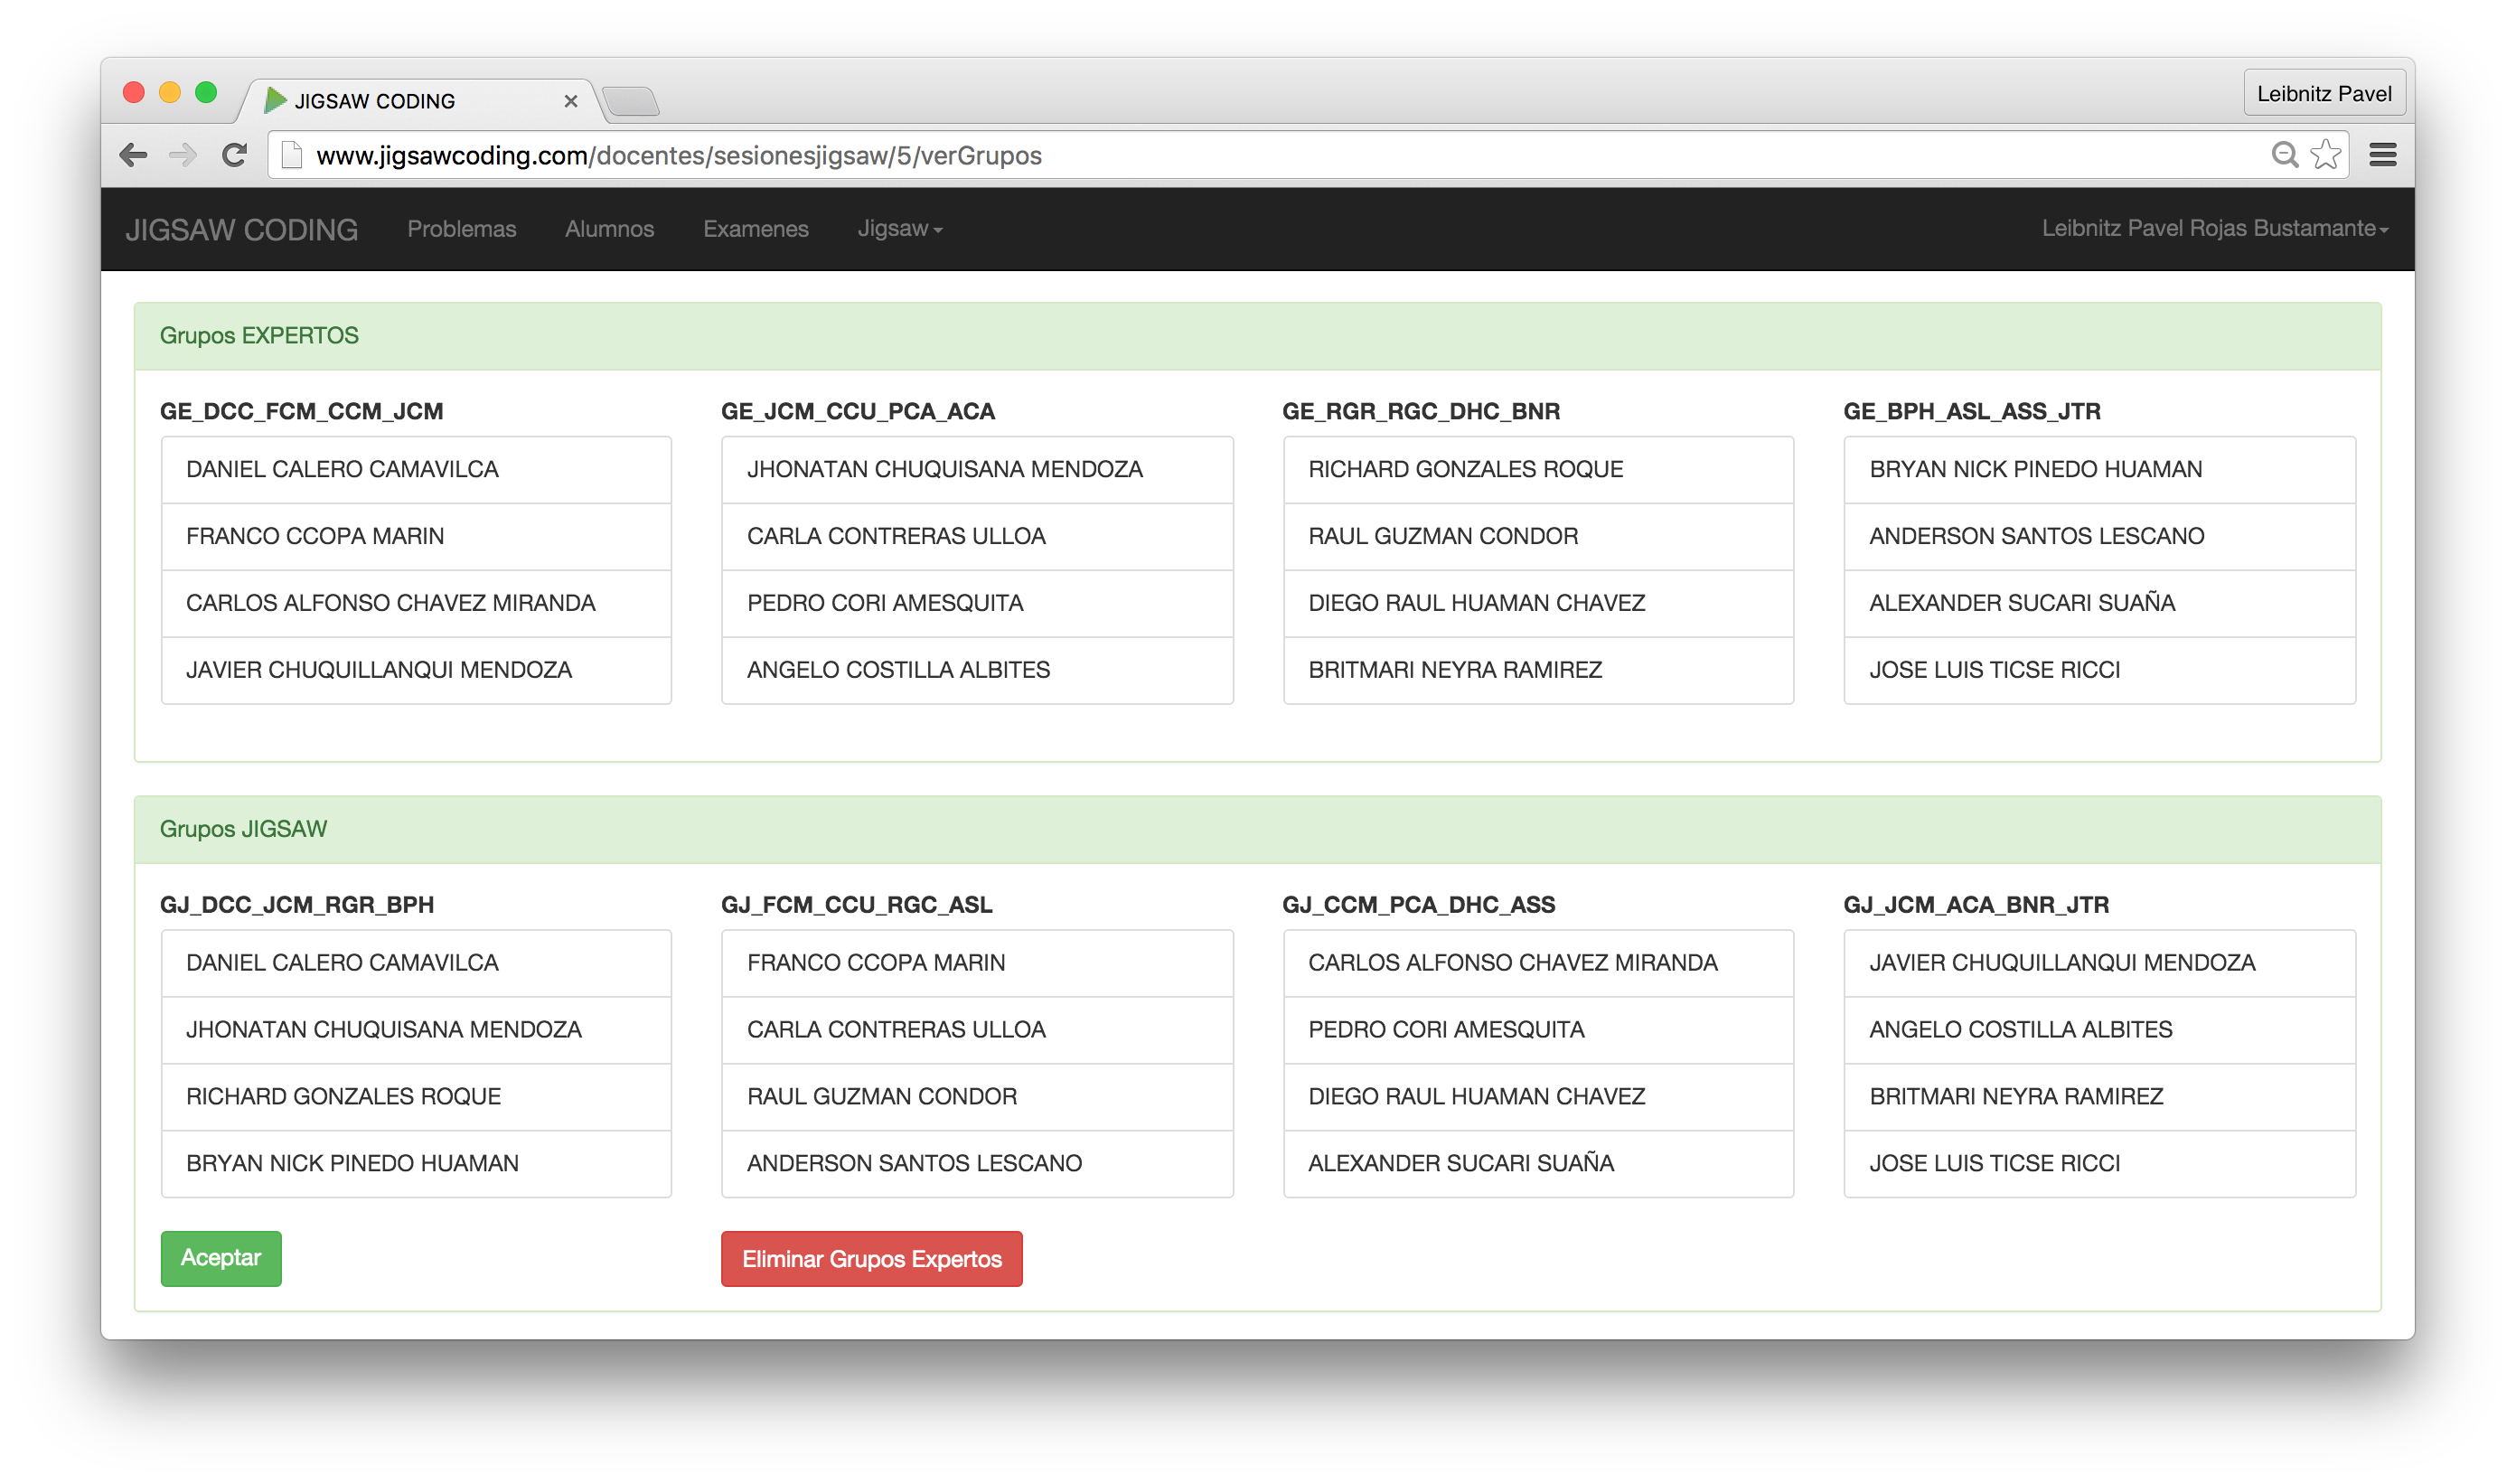
\includegraphics[scale=0.1]{figuras/chapter05/c5_sistemas_grupos}}
\end{figure}

En cuanto a la muestra con alumnos la EAP de Software, se formaron 3 grupos expertos y 3 grupos jigsaw tal y como puede apreciarse en la figura \ref{fig:c5_software_grupos}.

\begin{figure}[!h]
	\centering
	\caption{Grupos Expertos y Grupos Jigsaw - EAP Software}
	\label{fig:c5_software_grupos}
	\fbox{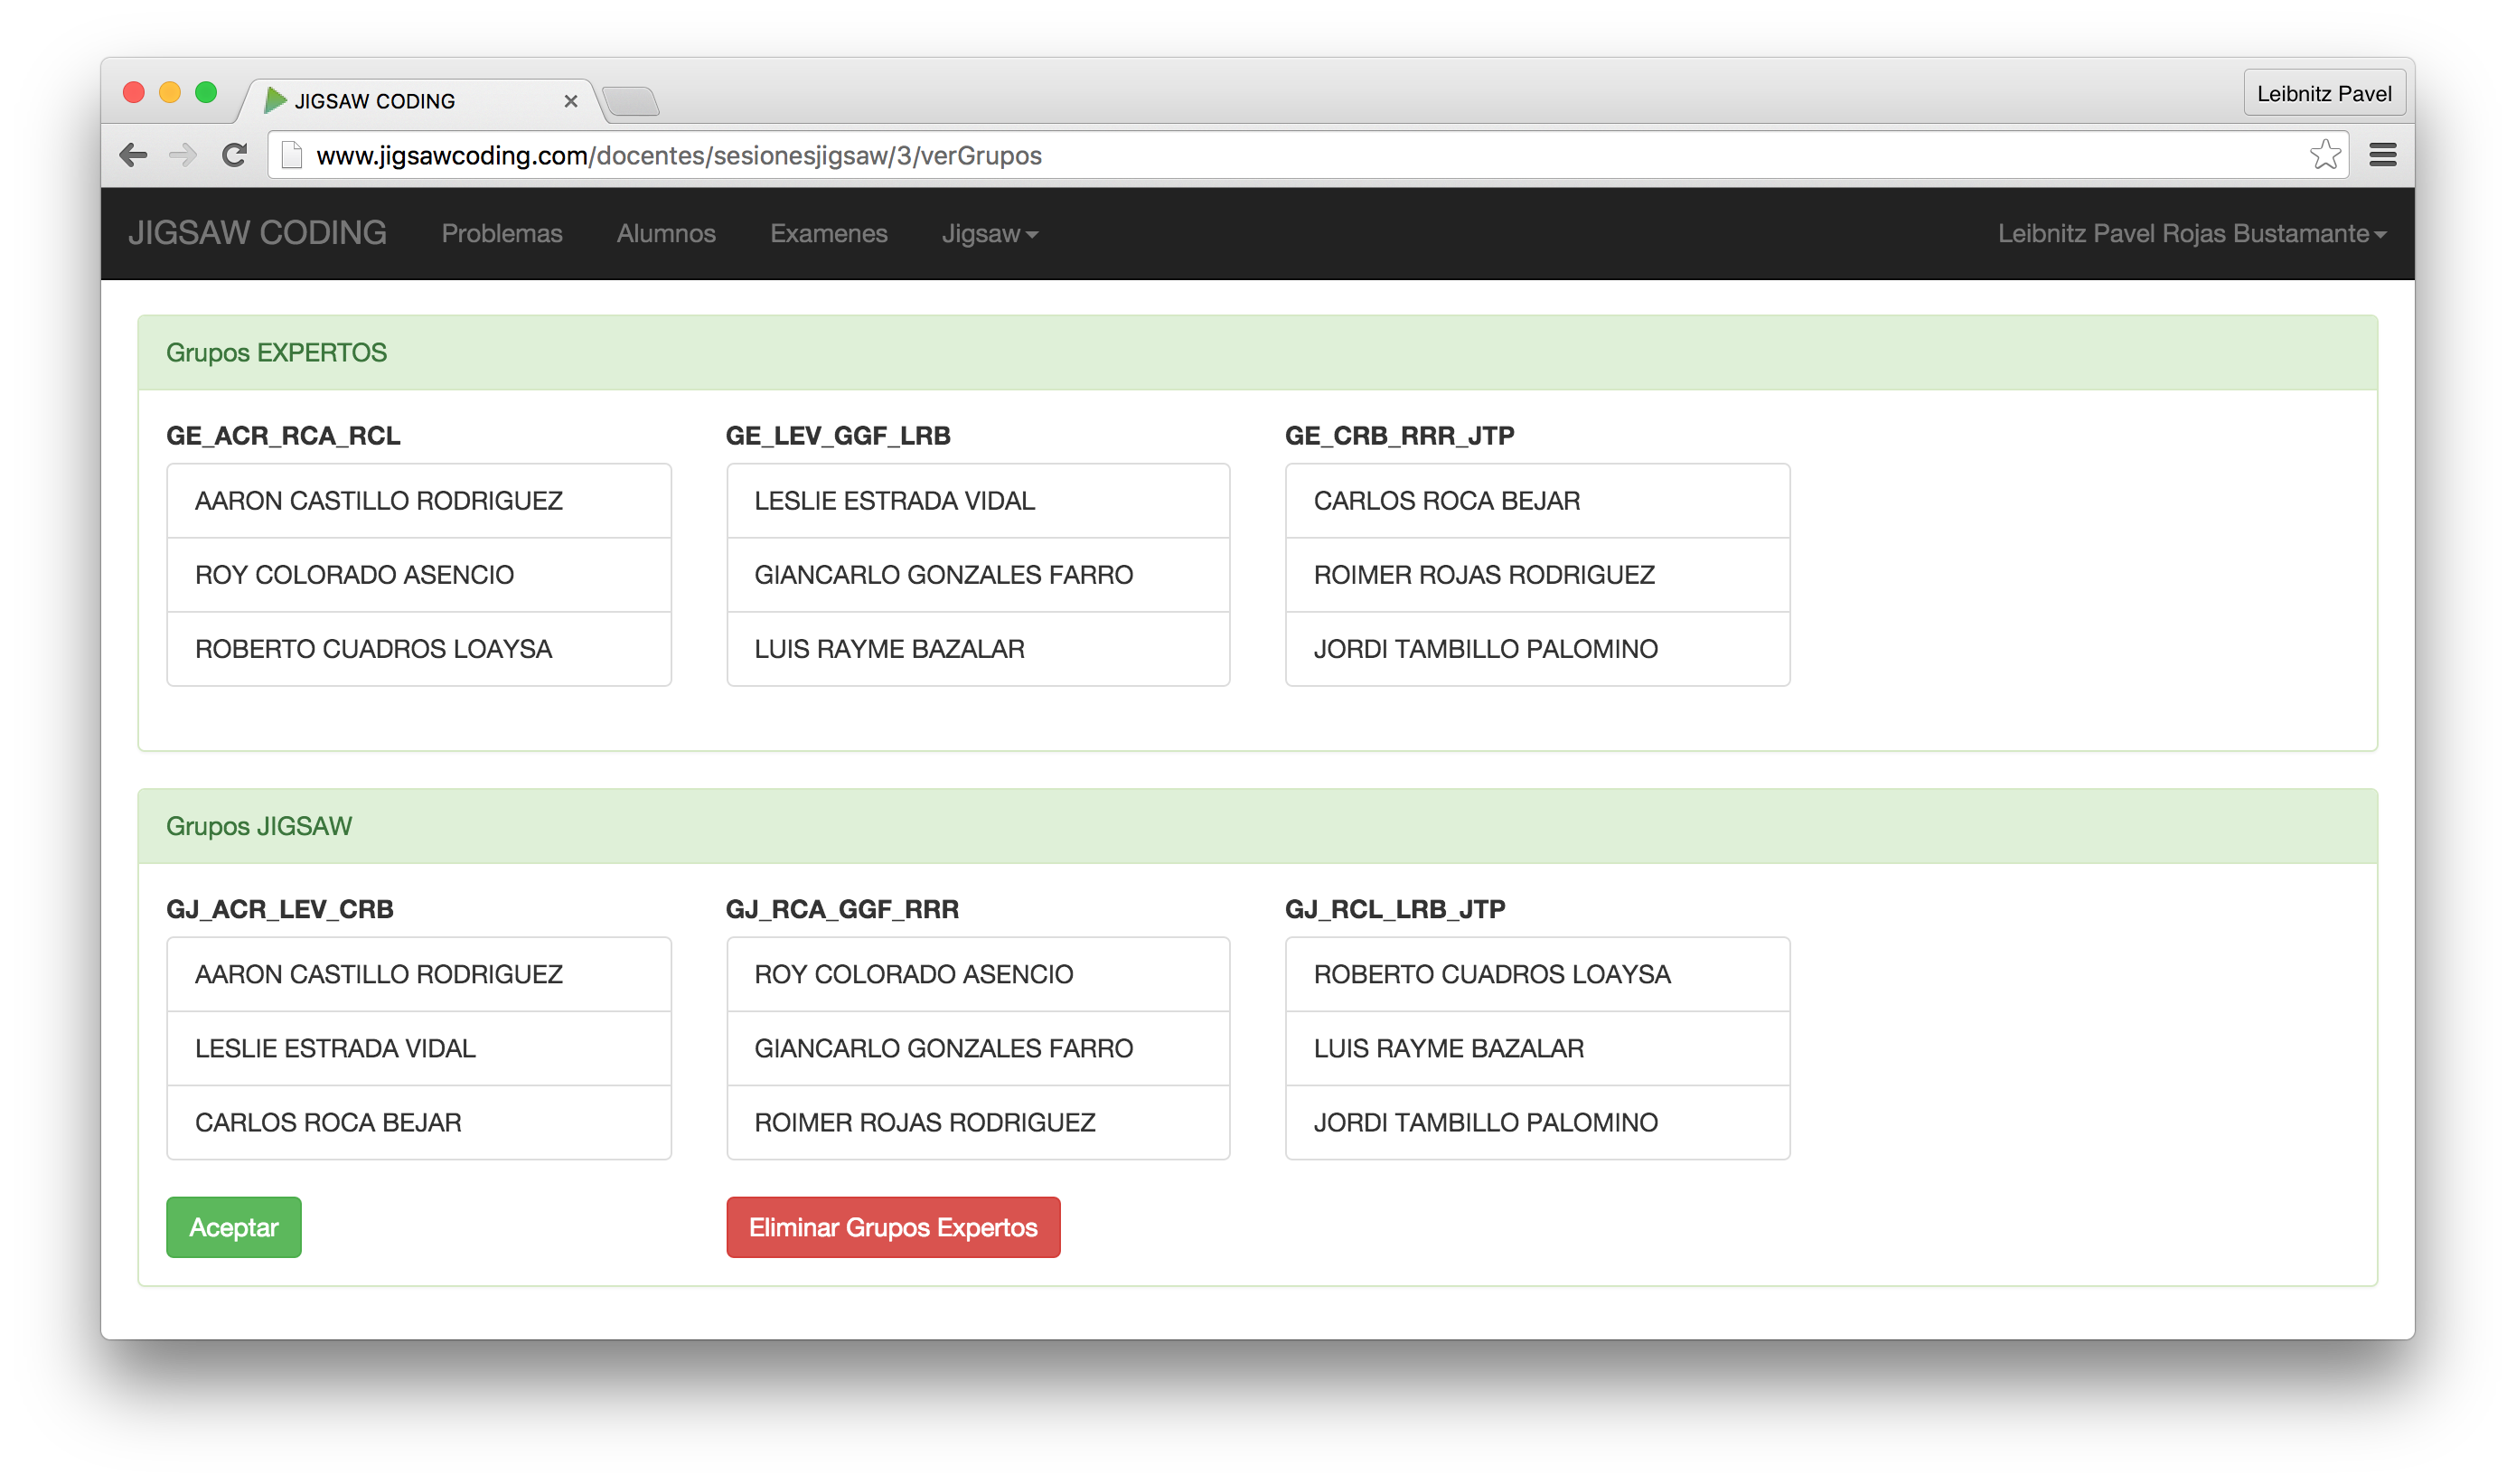
\includegraphics[scale=0.1]{figuras/chapter05/c5_software_grupos}}
\end{figure}

Las sesiones para Sistemas y Software se realizaron el día domingo 15 de noviembre del 2015. La hora de inicio y duración de cada una de las fases puede verse en las figuras \ref{fig:c5_sistemas_sesiones} y \ref{fig:c5_software_sesiones}. Cabe resaltar que en ambas figuras se muestra también la hora de inicio del examen para los grupos control. 

\begin{figure}[!h]
	\centering
	\caption{SJSistemas y SJSistemas-Control}
	\label{fig:c5_sistemas_sesiones}
	\fbox{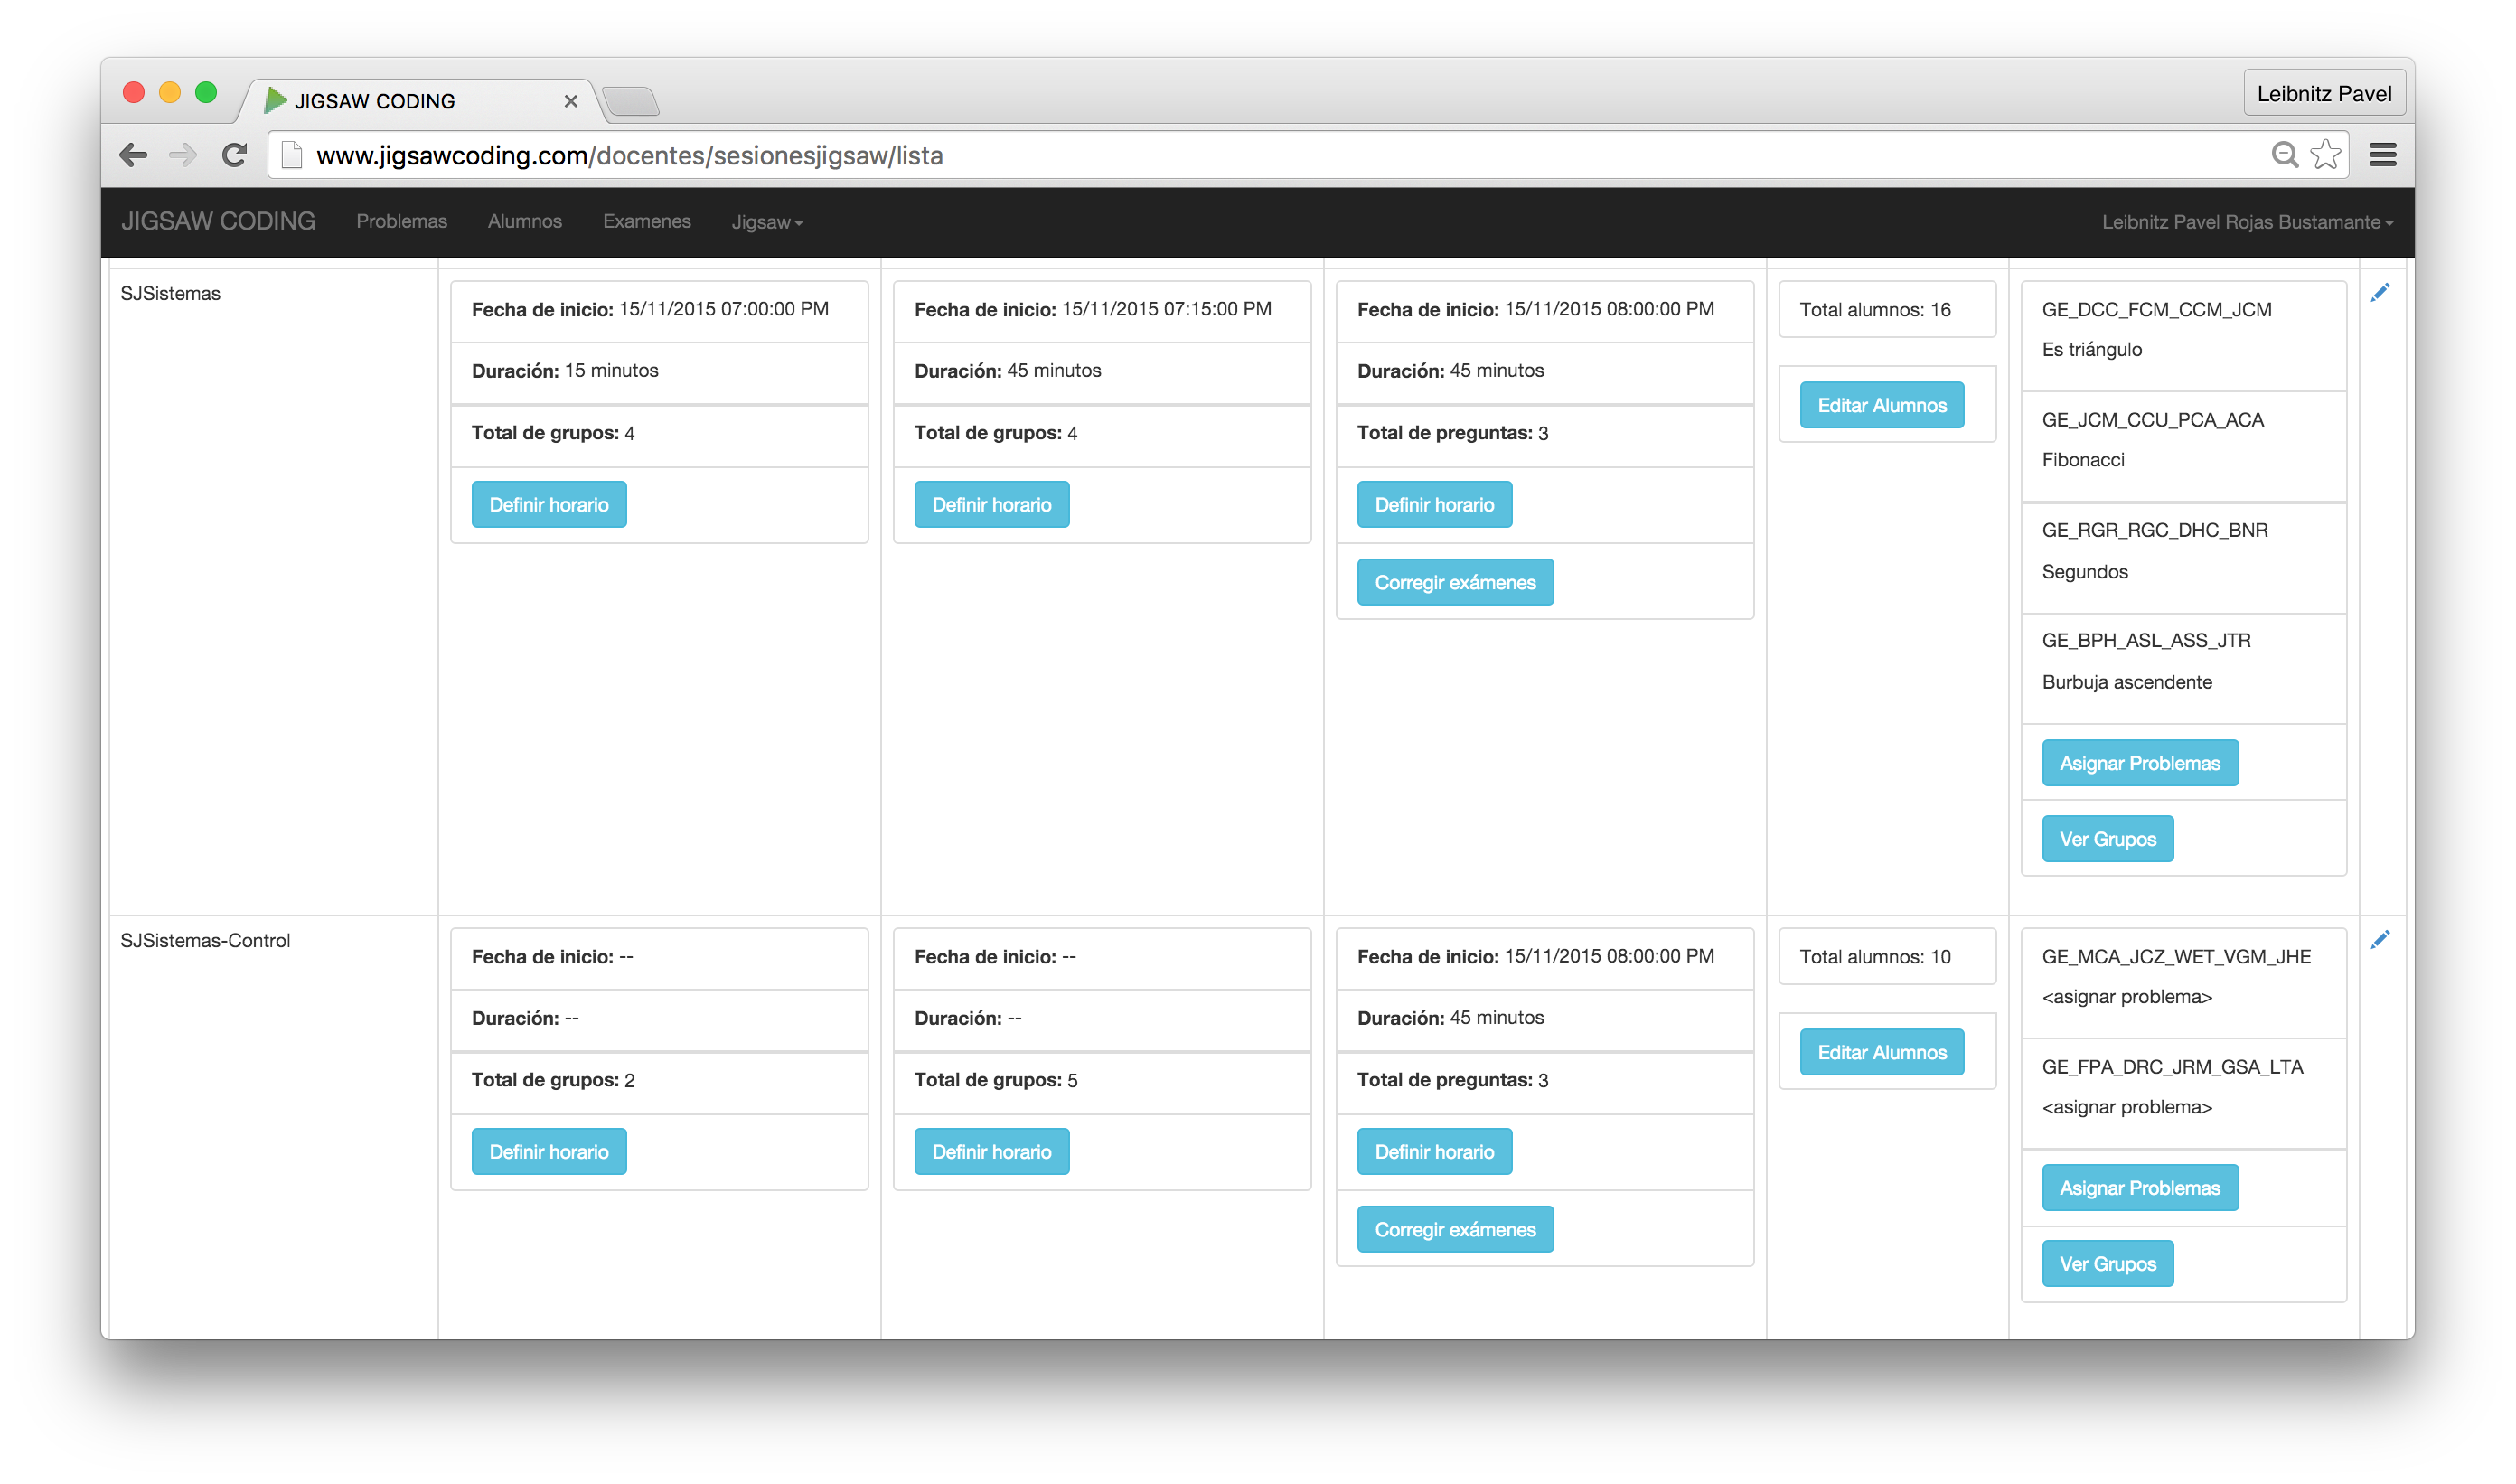
\includegraphics[scale=0.15]{figuras/chapter05/c5_sistemas_sesiones}}
\end{figure}

\begin{figure}[!h]
	\centering
	\caption{SJSoftware y SJSoftware-Control}
	\label{fig:c5_software_sesiones}
	\fbox{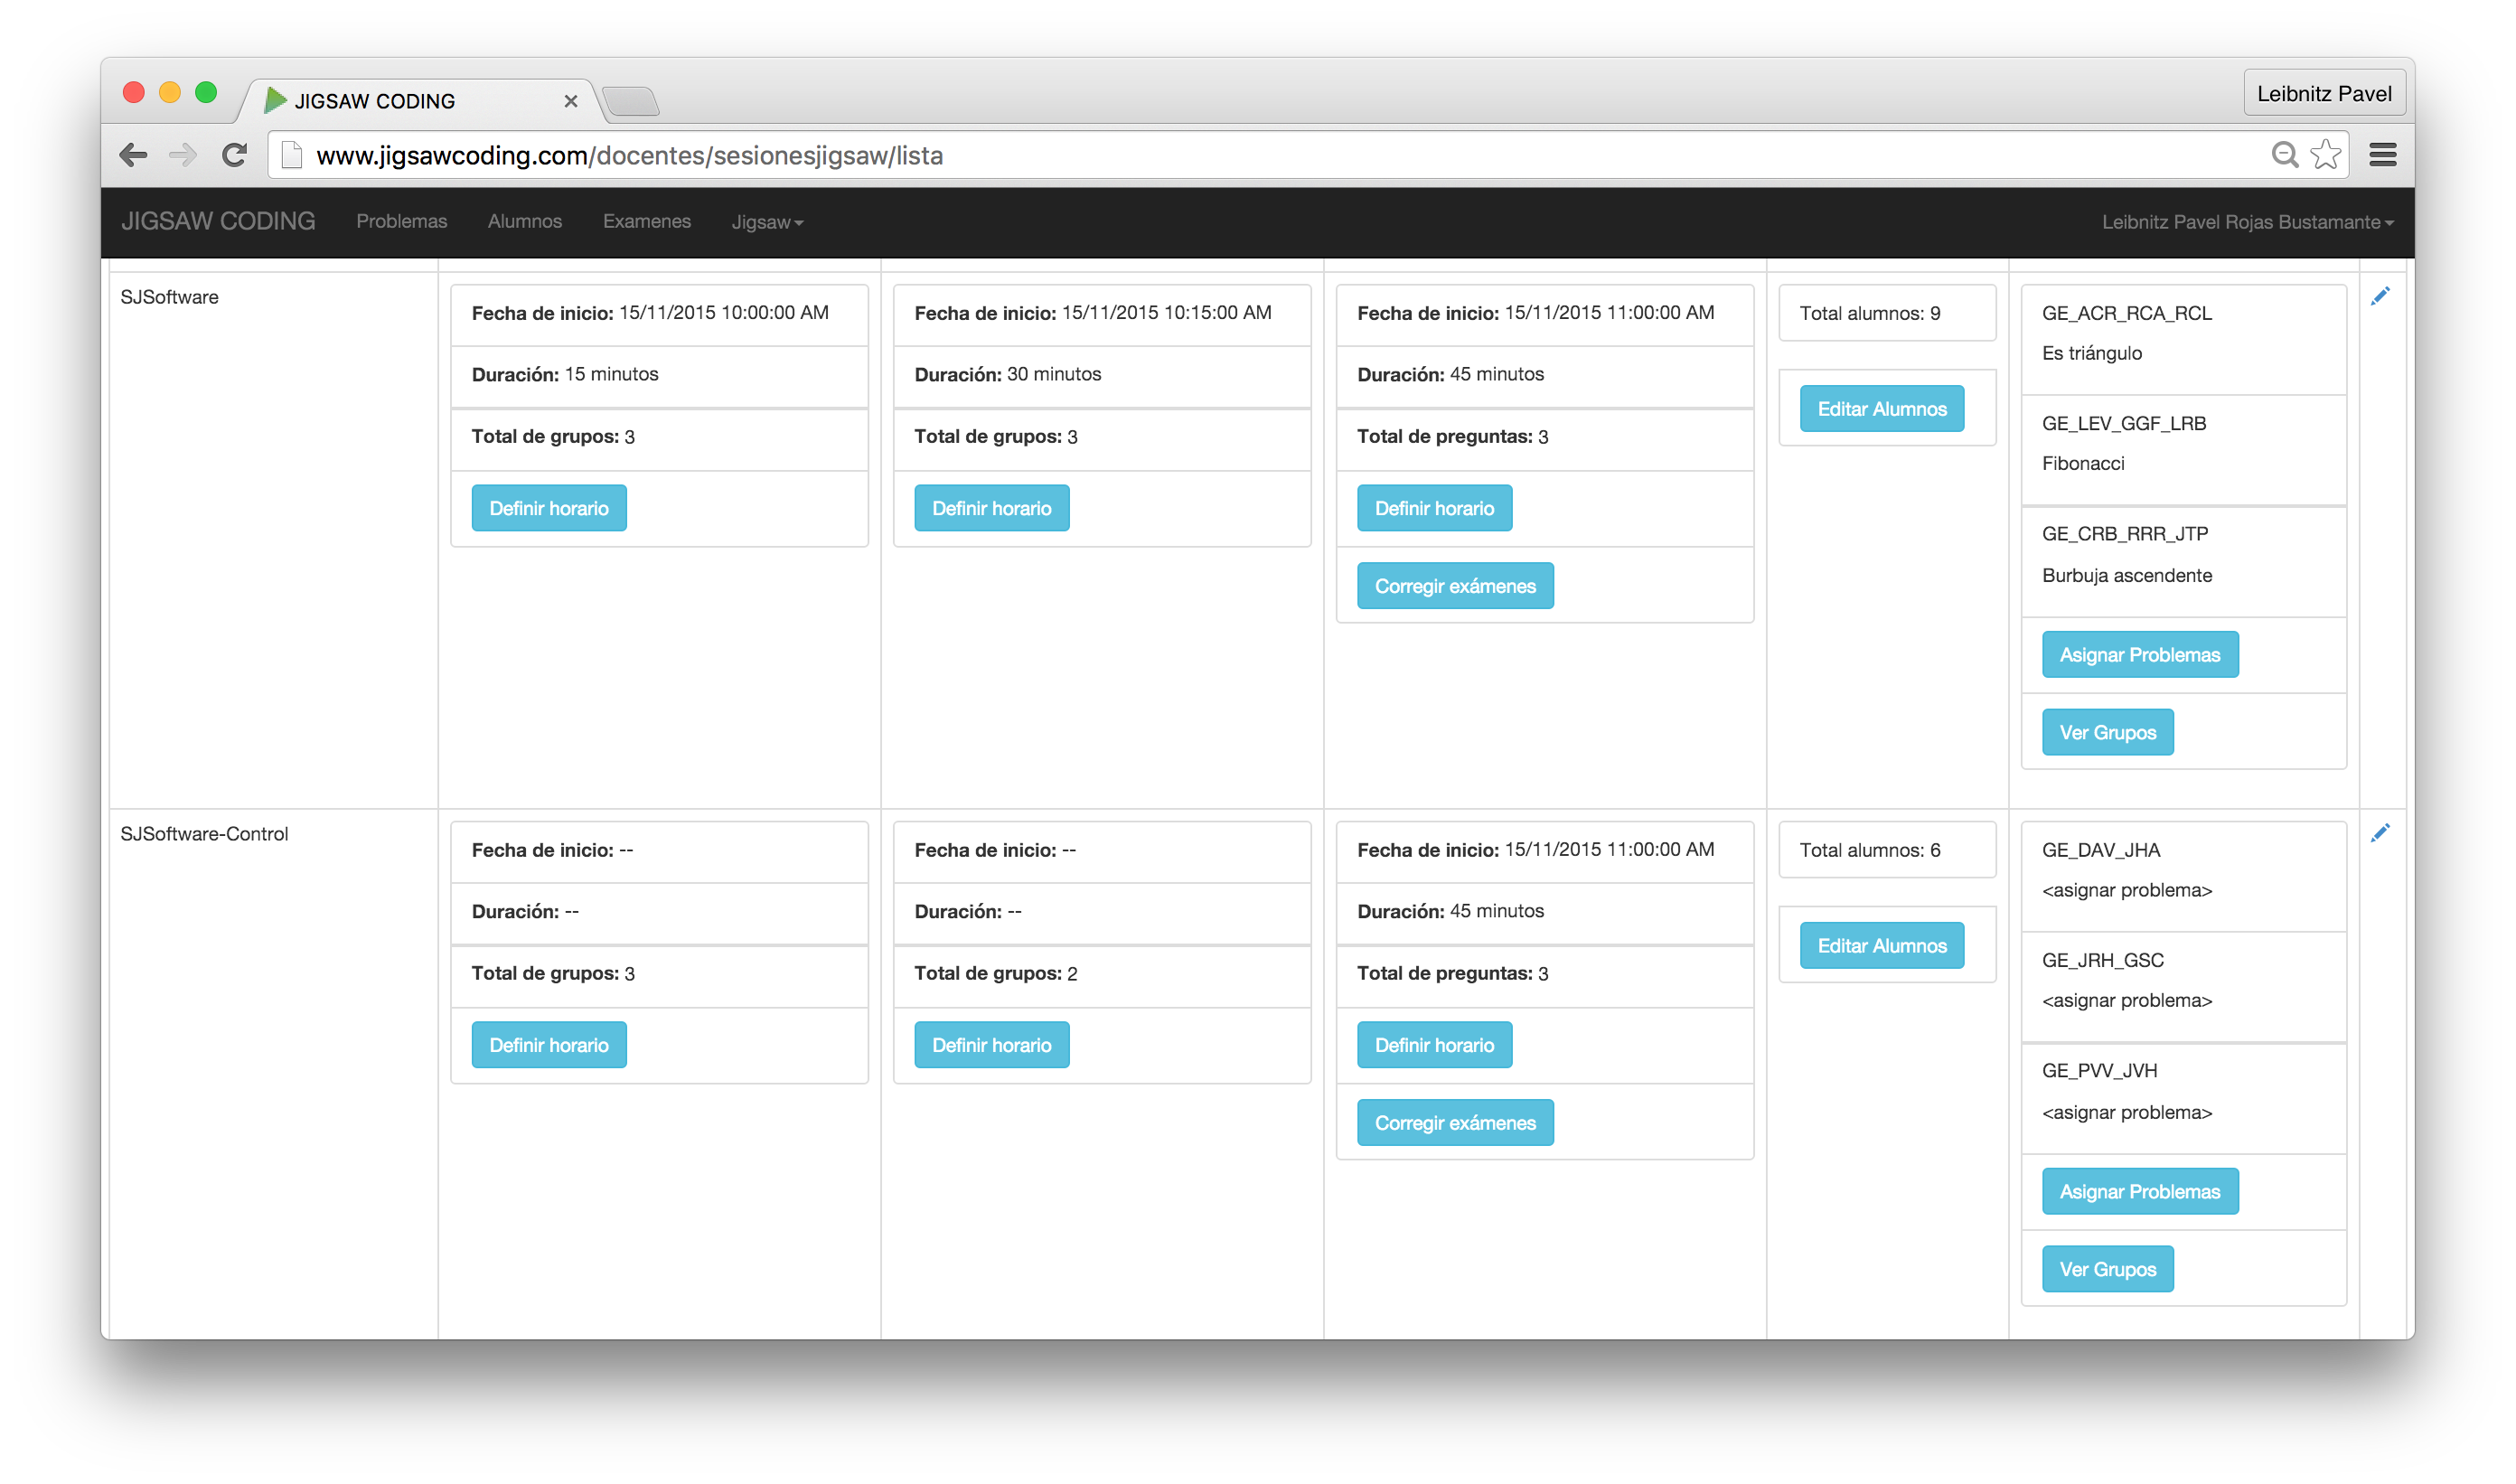
\includegraphics[scale=0.15]{figuras/chapter05/c5_software_sesiones}}
\end{figure}

Como se mencionó anteriormente, todos los 41 fueron evaluados con un examen que constaba de 3 preguntas: una de estructuras condicionales, una sobre recursividad y la tercera sobre ordenamiento. El examen fue elaborado también en el sistema JigsawCoding( Ver figura \ref{fig:c5_software_examen}).

\begin{figure}[!h]
	\centering
	\caption{Examen EAP Software}
	\label{fig:c5_software_examen}
	\fbox{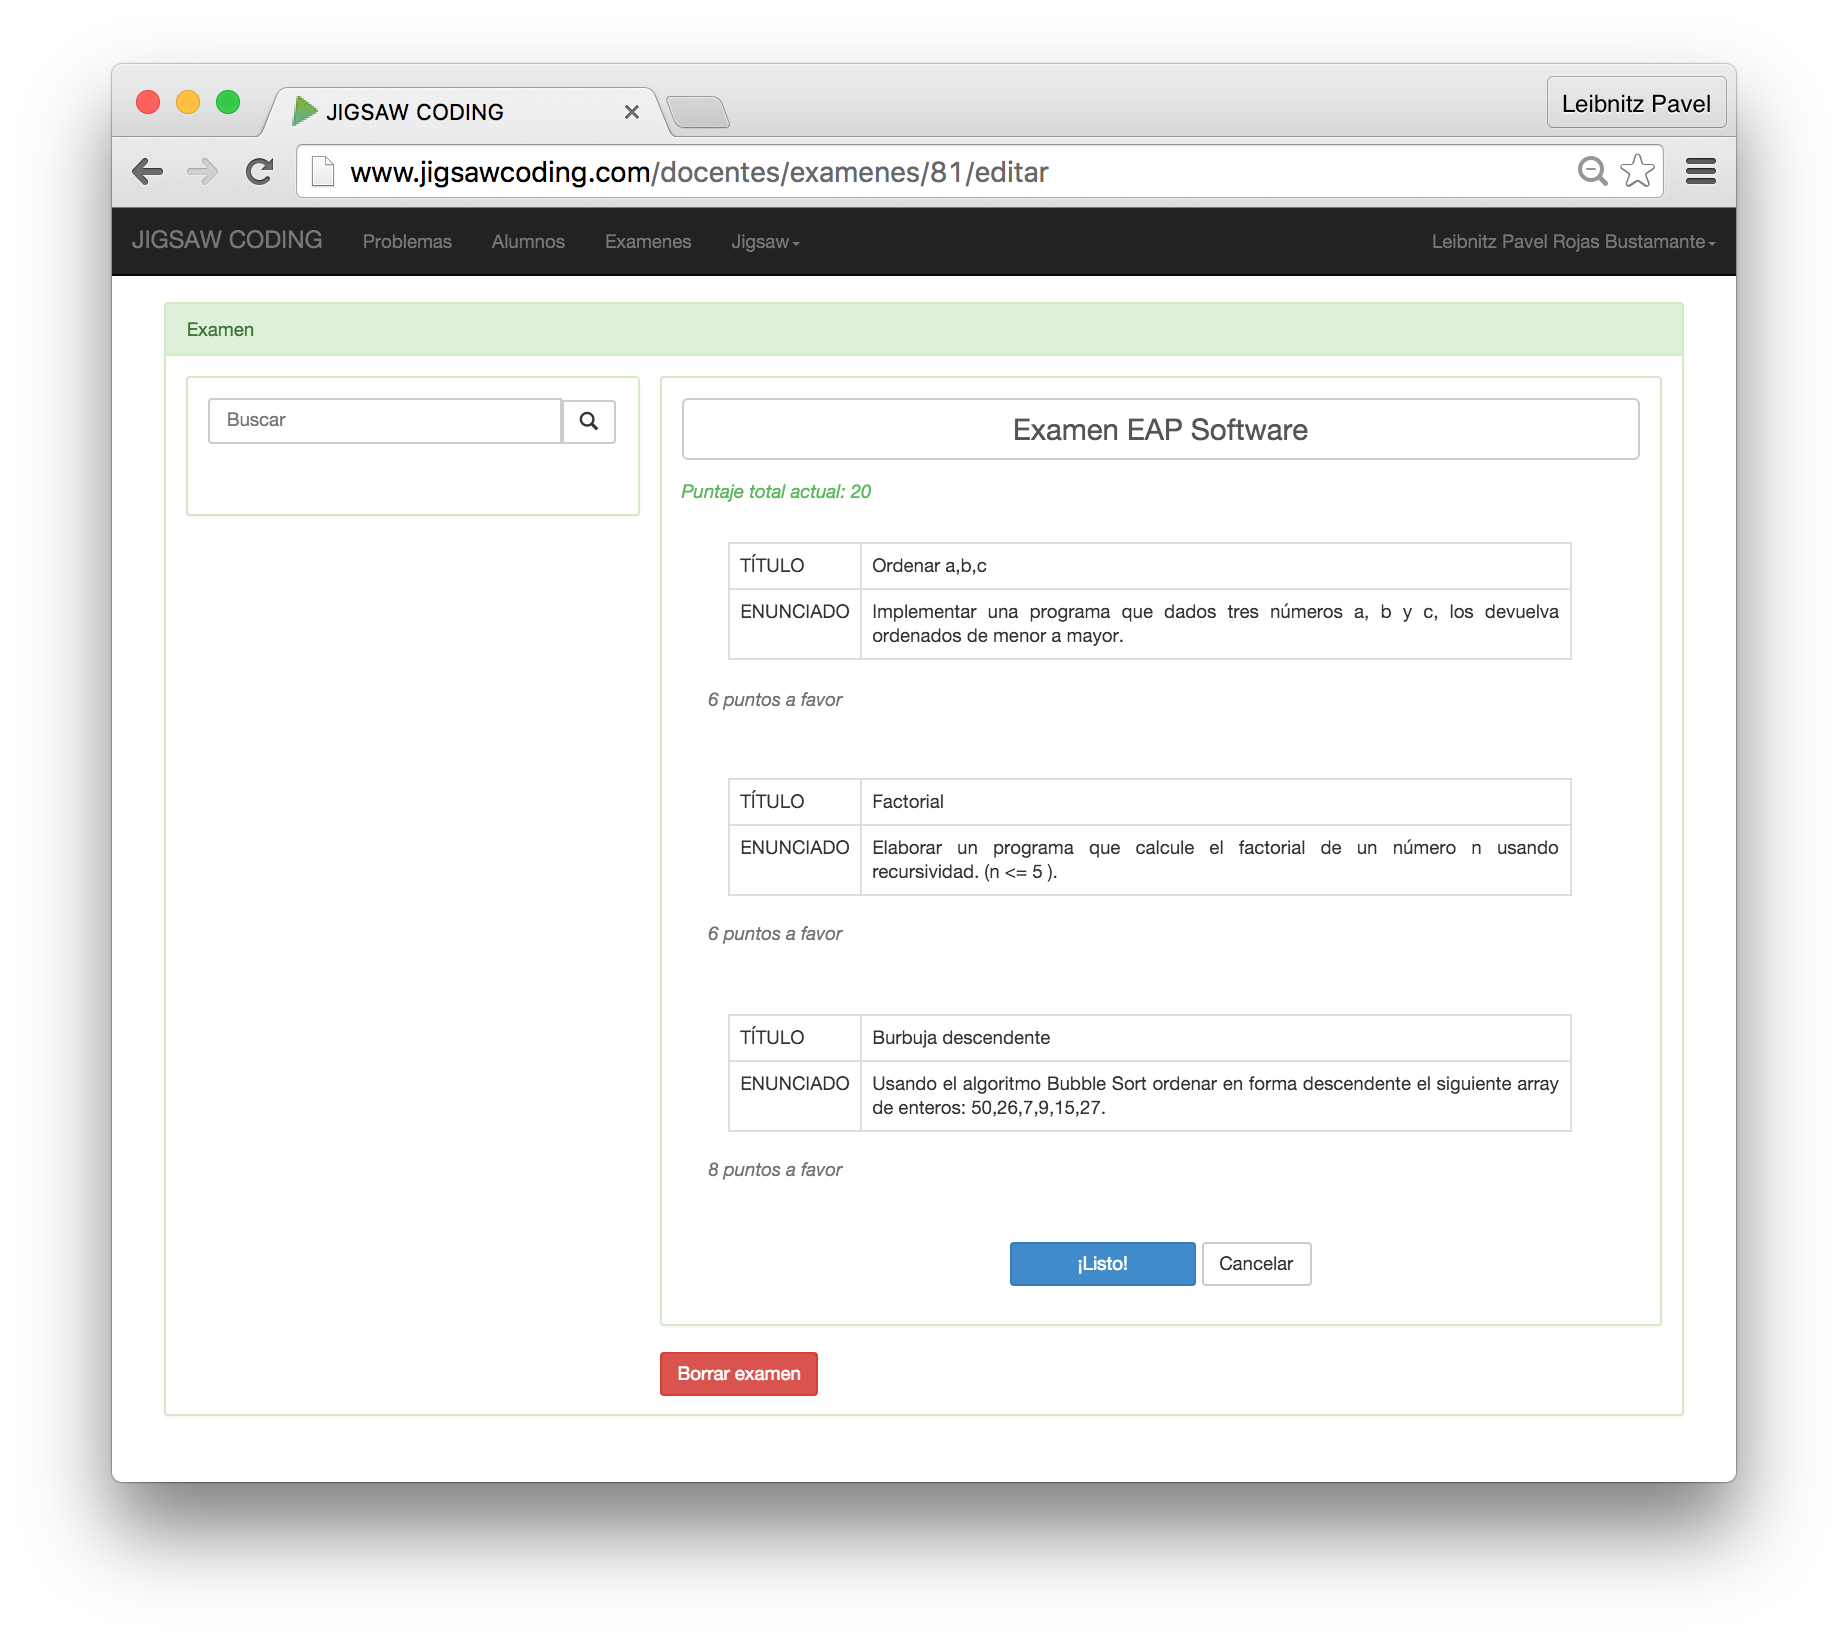
\includegraphics[scale=0.2]{figuras/chapter05/c5_software_examen}}
\end{figure}
